Die \emph{Cascade-Correlation Learning Architecture} ist eine von Scott Fahlman und Christian Lebiere entwickelte Architektur Neuronaler Netze, die sich in einigen Punkten von den bisher behandelten Modellen unterscheidet: Cascade-Correlation bestimmt nicht nur die Gewichte in einem Netzwerk mit festgelegter Topologie, sondern \emph{legt die Topologie des Netzwerks
mit fest}. Es beginnt mit einem minimalen Netz und fügt während des Trainings jeweils neue verdeckte Neuronen (hidden units) einzeln hinzu.
Sobald ein neues verdecktes Neuron zum Netzwerk hinzugefügt wird, werden seine Eingangsgewichte eingefroren, so dass dieses Neuron ein Detektor für ein spezielles Teilmuster in der Eingabe bleibt.

Die Cascade-Correlation-Architektur baut damit sehr schnell Netze mit vielen Ebenen auf, die aber immer nur \emph{ein Neuron pro Ebene} besitzen.
Die Vorteile dieser Architektur sind:
\begin{itemize}
	\item Das Lernverfahren lernt Gewichte, \emph{sowie} Größe und Topologie des Netzes.
	\item Behält einmal gelernte Strukturen bei Änderung der Trainingsmenge bei (Stabilität).
	\item Keine Rückwärtspropagierung der Fehlersignale nötig.  
\end{itemize}

Es ist damit für einige Probleme sehr viel schneller als Varianten von Backpropagation.


\subsection*{Das Moving-Target-Problem}
Eines der Probleme von Backpropagation, das Anlass zur Entwicklung von Cascade-Correlation gab, war das \emph{Moving-Target-Problem}: Jedes verdeckte Neuron eines mehrstufigen feedforward-Netzes versucht beim Training gleichzeitig mit den anderen Neuronen zu einem "`nützlichen"' Detektor für ein Teilmuster (\emph{feature}) zu werden, indem es seine Eingangsgewichte entsprechend anpasst.
Diese Aufgabe wird ihm aber dadurch erschwert, dass sich alle anderen Neuronen gleichzeitig ebenfalls ändern. Die Neuronen einer verdecken Schicht können nicht direkt miteinander kommunizieren, jedes Neuron sieht nur seine eigenen Vorgängerneuronen und die von den Nachfolgeneuronen zurückpropagierten Fehler.
Dieses Fehlersignal ist das Problem, welches das einzelne Neuron zu lösen (minimieren) versucht, wobei sich aber der Fehlervektor durch die gleichzeitige Adaption aller anderen Neuronen ständig ändert. Diese gleichzeitige Änderung aller Neuronen erschwert die Anpassung für jedes einzelne Neuron.

Eine Möglichkeit, dieses Problem zu beheben, ist, nur wenige Gewichte des Netzwerks gleichzeitig zu ändern und den Rest konstant zu halten.
Cascade-Correlation verwendet ein Extrem dieser Strategie, indem es nur die Gewichte \emph{eines} Neurons zu jedem Zeitpunkt ändert.
Man könnte glauben, dass diese Strategie die Geschwindigkeit des Lernens vermindert, aber Messergebnisse zeigen, dass Cascade-Correlation damit für viele Probleme schneller lernt als die bekannten Varianten von Backpropagation.

\subsection*{Der Cascade-Correlation-Algorithmus}
Der Cascade-Correlation-Algorithmus lässt sich durch zwei Ideen charakterisieren:
\begin{enumerate}
	\item \emph{Kaskaden-Architektur} - In ihr werden verdeckte Neuronen einzeln zum Netzwerk hinzugefügt und ihre Eingangsgewichte danach nicht mehr verändert.
	\item \emph{Lernalgorithmus} - Er erzeugt die versteckten Neuronen und bestimmt deren Gewichte so, dass der Betrag der Korrelation zwischen der Ausgabe des Neurons und dem restlichen Fehlersignal maximal wird. So kann er den Restfehler möglichst stark minimieren.
\end{enumerate}

\subsubsection*{Kaskaden-Architektur}
Die Architektur eines Cascade-Correlation-Netzes ist in Abbildung \ref{fig:ch06_cascade-correlation} dargestellt.

\begin{figure}[ht!] \centering 
	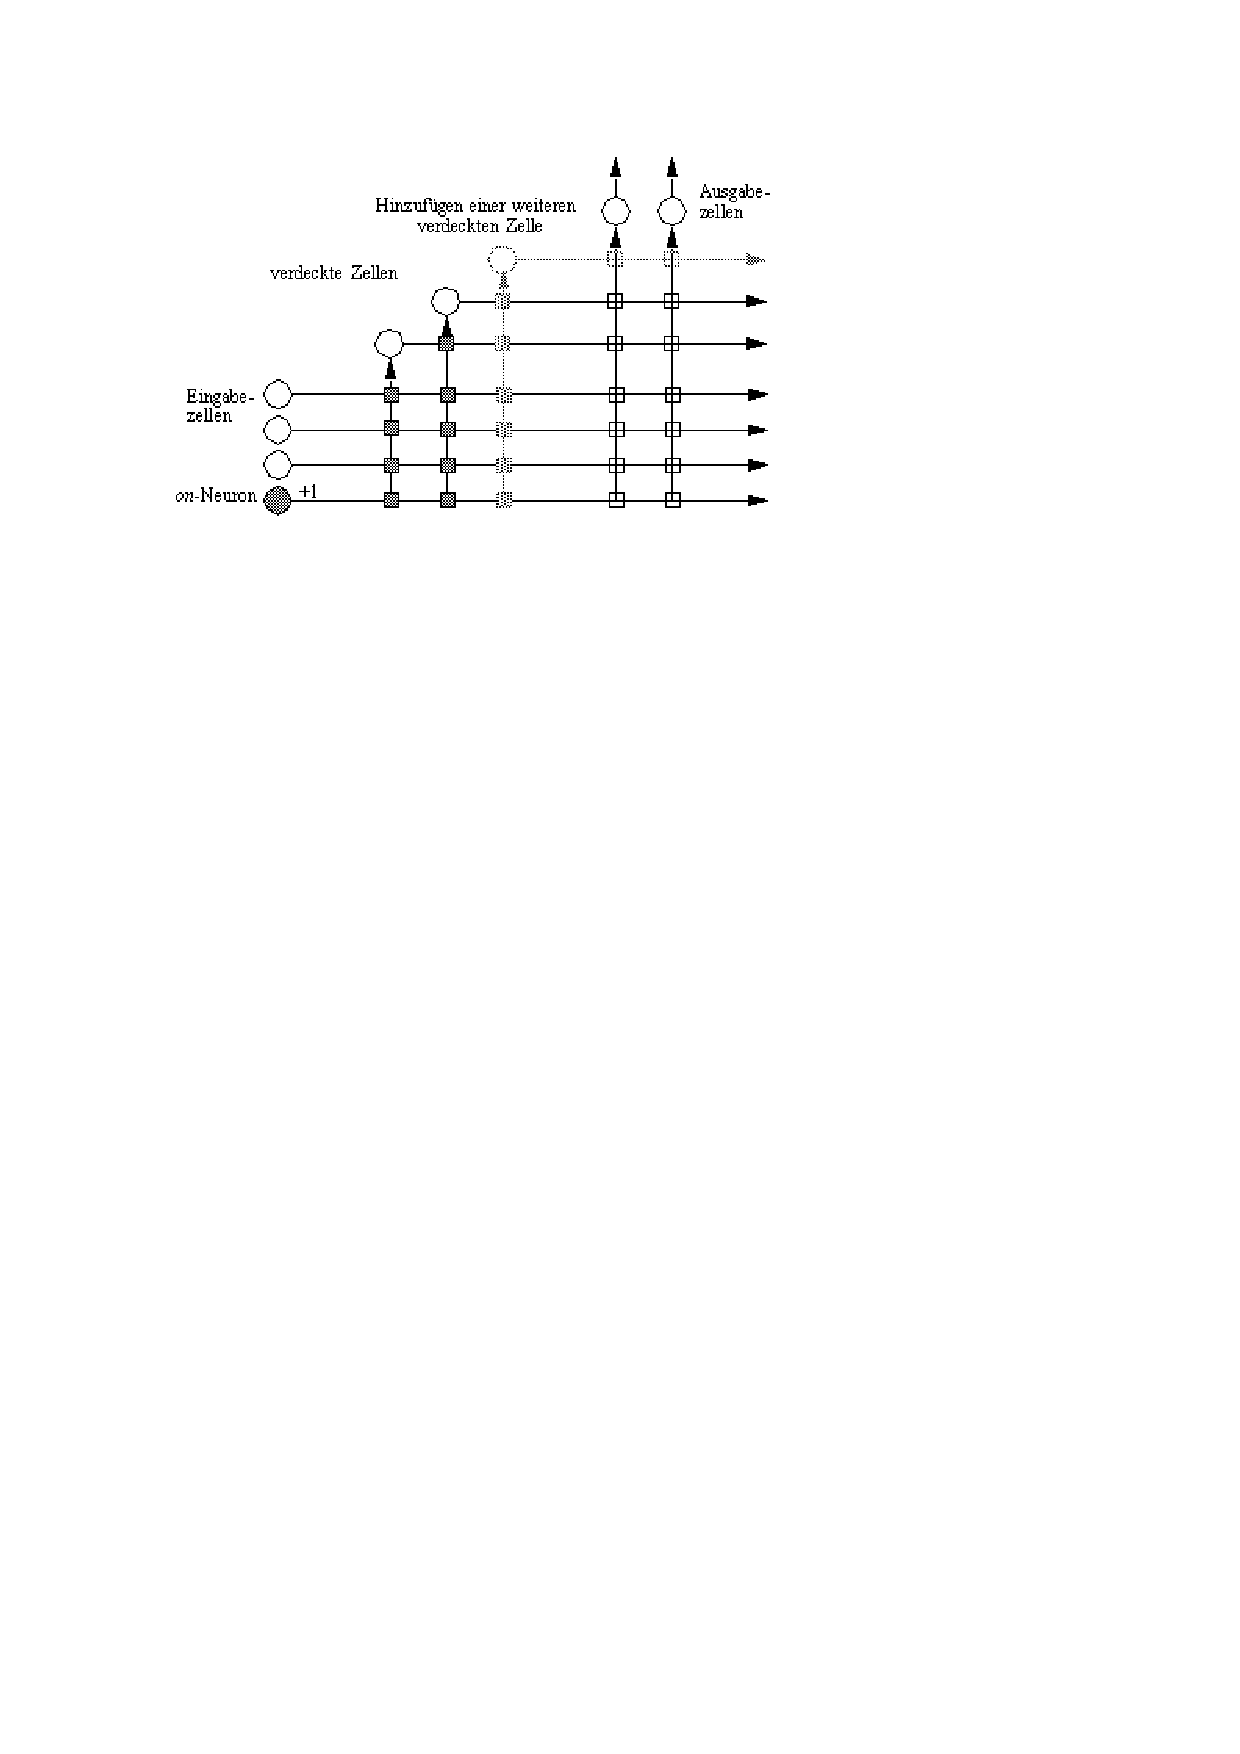
\includegraphics[width=\linewidth]{figures/ch06_cascade-correlation.pdf}
	\caption{Beispielhafte Cascade-Correlation"--Architektur, vor dem Hinzufügen des dritten verdeckten Neurons. Die vertikalen Verbindungen summieren alle Eingaben auf. Die Gewichte $w_{ij}$ sind als kleine Quadrate dargestellt. Dunkle Quadrate symbolisieren eingefrorene Gewichte, helle Quadrate sind Gewichte, die noch weiter trainiert werden.}
	\label{fig:ch06_cascade-correlation}
\end{figure}

Zu Beginn des Trainings existiert nur die durch die Problemstellung vorgegebene Anzahl von Eingabe- und Ausgabezellen, jedoch keine verdeckten Neuronen. Jede Eingabezelle ist mit jeder Ausgabezelle durch eine Verbindung mit trainierbarem Gewicht verbunden (helle Quadrate). Es existiert auch ein "`on"'-Neuron, dessen Ausgabe immer $+1$ ist und das mit allen Ausgabezellen verbunden ist, oder alternativ ein Schwellenwert in jeder dieser Zellen.
Die Ausgabeneuronen können eine lineare oder eine nichtlineare Aktivierungsfunktion besitzen\footnote{Die meisten Experimente mit Cascade-Correlation wurden bisher mit sigmoiden Aktivierungsfunktionen wie tangens hyperbolicus $tanh(x)$ oder der logistischen Aktivierungsfunktion durchgeführt.}.


\subsection*{Lernalgorithmus}
Das Lernverfahren fügt nun einzeln verdeckte Neuronen zu dem Netzwerk hinzu.
\begin{itemize}
	\item Jedes neue Neuron erhält Eingaben von \emph{allen} Vorgängern (Eingabeneuronen und vorher generierte versteckte Neuronen).
	\item Die Eingabegewichte jedes neuen Neurons werden eingefroren.
	\item Nur Gewichte zu den Ausgabeneuronen werden weiter trainiert.
\end{itemize}

Auf diese Art und Weise stellt jedes Neuron der verdeckten Schicht eine Ebene für sich dar. Dies führt zur Erzeugung sehr mächtiger Detektoren für Teilmuster höherer Ordnung, hat jedoch den Nachteil, dass das erzeugte Netzwerk recht tief ist und verdeckte Neuronen einen immer größeren "`fan-in"' erhalten.

Der Lernalgorithmus beginnt zuerst ohne verdeckte Neuronen. Die direkten Verbindungen zwischen Eingabeebene und Ausgabeebene werden über die gesamte Trainingsmenge so gut wie möglich trainiert, beispielsweise durch die Delta-Regel (Widrow-Hoff-Regel) oder durch Quickprop.

Sobald über eine Anzahl von Zyklen keine deutliche Änderung des Fehlers mehr zu beobachten ist wird das Netzwerk ein letztes Mal mit der gesamten Trainingsmenge getestet und der kumulierte Fehler gemessen. 

\begin{itemize}
	\item Ist dieser klein genug, terminiert das Verfahren ohne Erzeugung verdeckter Neuronen mit einem einstufigen Netzwerk (einer Ebene trainierter Gewichte zwischen Eingabe und Ausgabe).
	\item Im anderen Fall gibt es einen Restfehler, der durch Einführung eines oder mehrerer verdeckter Neuronen reduziert werden muss. Es wird ein neues verdecktes Neuron dem Netz hinzugefügt, dessen Gewichte der Eingangsverbindungen wie nachfolgend beschrieben bestimmt werden. \\
	Dieser Vorgang des Hinzufügens wird wiederholt, bis der Fehler klein genug ist (oder bis die maximal tolerierbare Zeit zum Training überschritten wurde).
\end{itemize}

Zur Erzeugung einer neuen verdeckten Zelle beginnt man mit einer \emph{Kandidatenzelle} $j$, die trainierbare Gewichte von allen Vorgängern erhält, während die Ausgabe noch nicht mit dem Netzwerk verbunden ist.
Nun erfolgt eine Anzahl Durchläufe durch die gesamte Trainingsmenge, wobei die Eingabegewichte wie folgt beschrieben geändert werden.

Ziel der Änderungen ist es, $S_j$, die Summe der Beträge der Korrelation\footnote{Genaugenommen ist $S$ nicht eine Korrelation, sondern eine Kovarianz, da einige Normalisierungsterme in der Formel fehlen. Tatsächlich funktioniert das Lernverfahren mit der hier angegebenen Kovarianz in den meisten Fällen sogar besser als mit der Korrelation.} zwischen $o_j$, der Ausgabe der Kandidatenzelle, und $\delta_k$,
dem Restfehler der Ausgabezelle $k$, über alle Ausgabezellen $k$ zu maximieren.
\[
	S_j = \sum_k \big | \sum_p (o_{pj} - \bar{o}_j) (\delta_{pk} - \bar{\delta_k}) \big |
\]
Dabei ist $j$ der Index der Kandidatenzelle, $k$ der Laufindex über alle Ausgabeneuronen, $p$ der Index der Muster, $\bar{o_j}$ die mittlere Ausgabe von Neuron $j$ über alle Muster $p$ und $\bar{\delta_{pk}}$ der mittlere Fehler von Ausgabezelle $k$ über alle Muster $p$.

Um $S_j$ zu maximieren, muss die partielle Ableitung $\frac{\partial S_j}{\partial w_{ij}}$ berechnet werden. Es gilt:
\[
	\frac{\partial S_j}{\partial w_{ij}} = 
		\sum_k \sum_p \sigma_k \cdot f'_{act}(net_{pj}) \cdot
		o_{pi} \cdot (\delta_{pk} - \bar{\delta{k}})
\]

Nachdem der Wert für $\frac{\partial S_j}{\partial w_{ij}}$ für jedes Gewicht von der Eingabezelle $i$ zu der Kandidatenzelle $j$ berechnet wurde, kann man einen \emph{Gradientenaufstieg} durchführen, um $S$ durch die Änderung der Verbindungsgewichte $w_{ij}$ zu maximieren.
Sobald sich $S$ nicht mehr erhöht, wird das neue verdeckte Neuron als Neuron in das aktive Netzwerk installiert, seine Eingabeverbindungen werden eingefroren und der oben beschriebene Zyklus wird fortgeführt.

Durch den Betrag in der Formel für $S_j$ versucht ein Neuron nicht das Vorzeichen, sondern nur den Betrag der Korrelation seiner Ausgabe mit dem Fehler der Ausgabeneuronen zu maximieren.
Wenn ein Neuron positiv mit dem Fehler einer Ausgabezelle korreliert, bildet es eine negative Verbindung zu dieser Ausgabezelle aus, die den Fehler vermindert; ist die Korrelation negativ, ist das Gewicht zum Ausgabeneuron positiv.

\subsubsection*{Kandidatengruppen}
Anstelle eines einzelnen Kandidatenneurons kann man auch eine Gruppe von Kandidatenneuronen trainieren\footnote{Üblich ist eine Gruppengröße von vier bis acht Kandidatenneuronen.}, jede mit einer anderen Menge von Initialgewichten. Da sie nichts miteinander zu tun haben, können alle Kandidatenneuronen \emph{parallel} trainiert werden.
Das Kandidatenneuron mit der besten Korrelation nach der Trainingsphase wird dann installiert.

Die Verwendung eine Gruppe von Kandidaten ist vorteilhaft:
\begin{itemize}
	\item Die Chance, dass ein nutzloser Kandidat, dessen Training selbst (in einem lokalen Maximum) hängen geblieben ist, permanent installiert wird, ist geringer.
	\item Das Training wird beschleunigt, weil mehrere Teile des Gewichtsraums parallel durchsucht werden können.
	\item Unterschiedliche Neuronen-Typen (z.B. sigmoid, Gauß, radial) innerhalb einer Gruppe können zu kompakteren und eleganteren Netzwerken führen.
\end{itemize}


\subsection*{Vergleich mit anderen Verfahren}
\subsubsection*{2-Spiralen-Problem}
Für den Vergleich von Cross Correlation und anderen Verfahren haben Fahlman und Lebiere das \emph{2-Spiralen-Problem} von A. Wieland genutzt.
Dieses Problem ist deshalb sehr schwer, weil durch die Verschränkung der Spirale ein feedforward-Netz mit sigmoiden Neuronen mehrere Ebenen verdeckter Neuronen und \emph{shortcut connetctions}\footnote{\emph{Shortcut connections} sind Verbindungen, welche Ebene des Netzes überspringen.} benötigt.
Abbildung \ref{fig:ch06_2-spiralen-problem} zeigt das 2-Spiralen-Problem und die von Cascade-Correlation gefundenen Separierung.

\begin{figure}[ht!] \centering 
	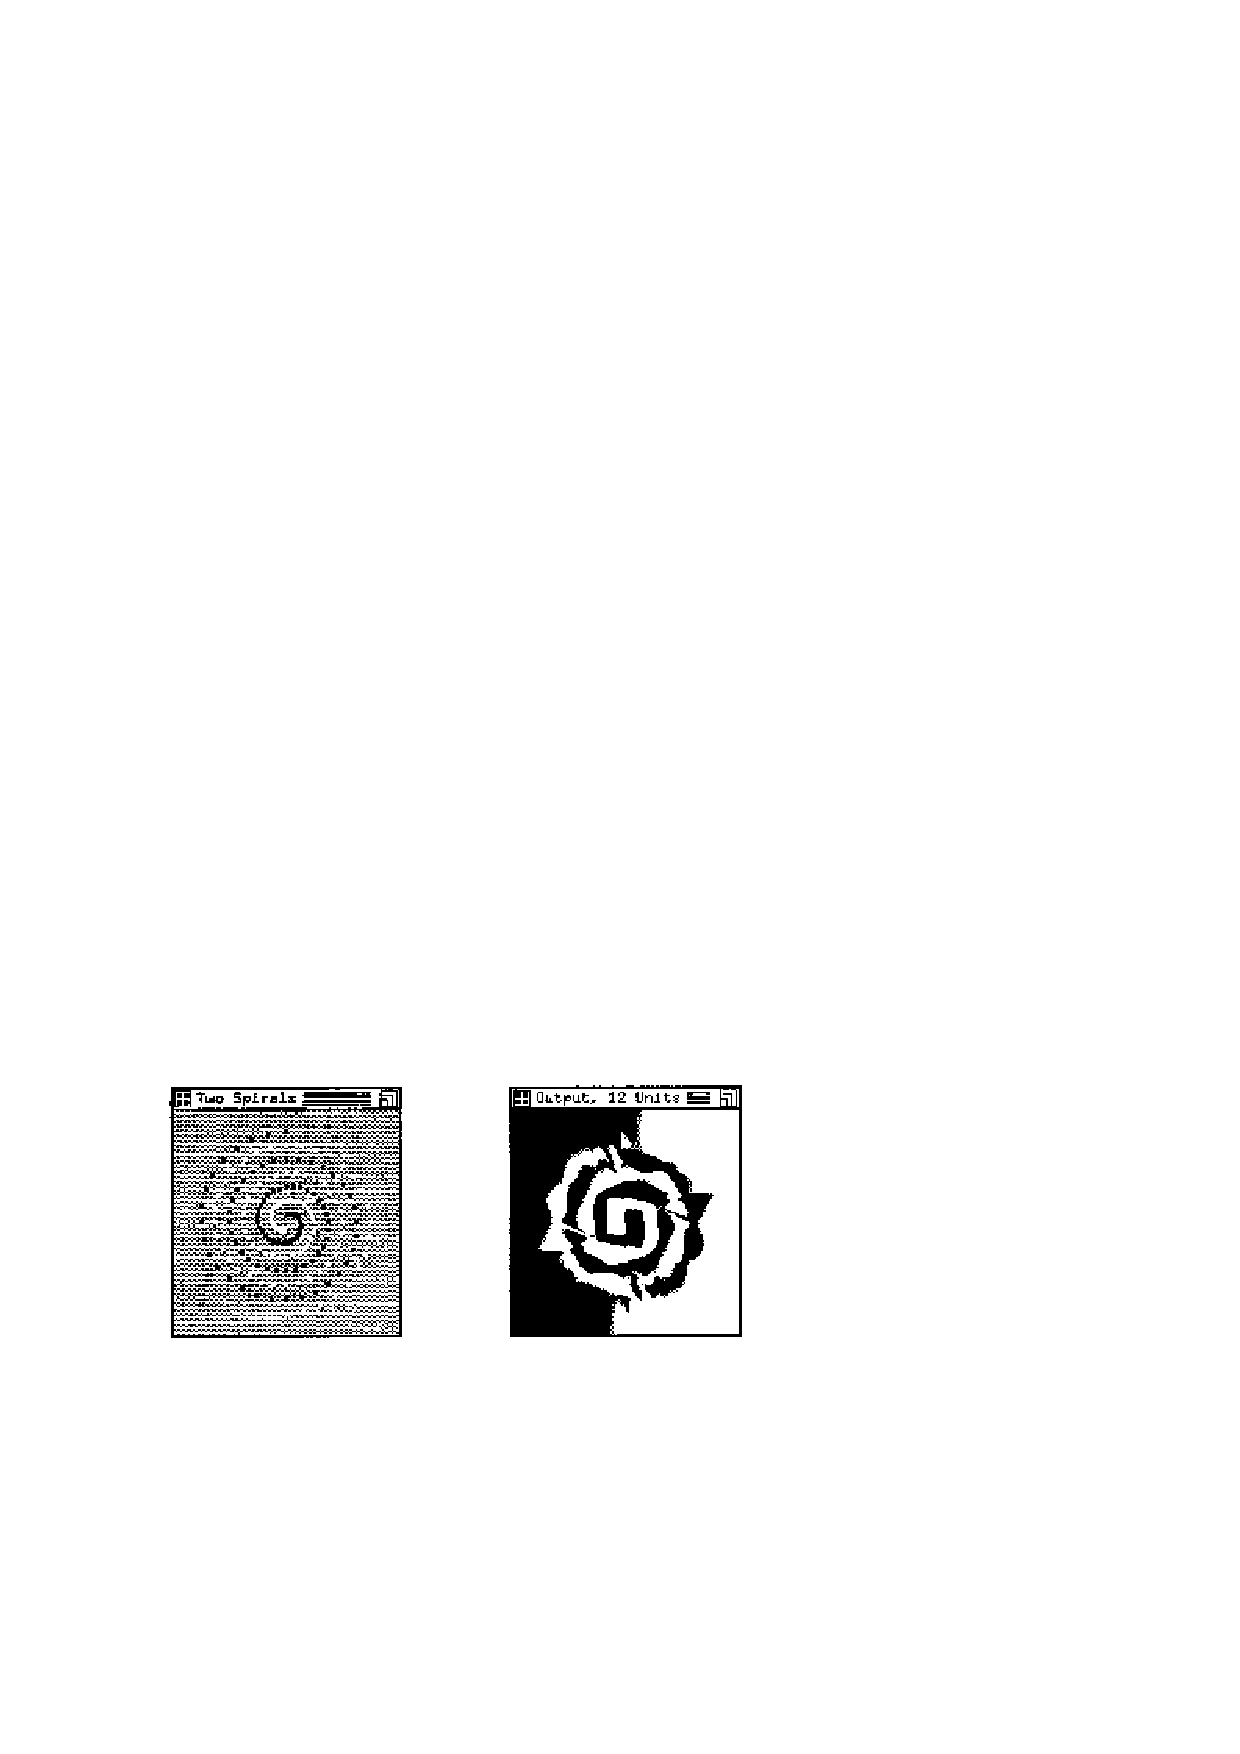
\includegraphics[width=\linewidth]{figures/ch06_2-spiralen-problem.pdf}
	\caption{Trainingspunkte des 2-Spiralen-Problems (links) und Ausgabe eines Netzwerks, das mit Cascade-Correlation trainiert wurde (rechts).}
	\label{fig:ch06_2-spiralen-problem}
\end{figure}

\subsubsection*{Ergebnisse}
Lang und Witbrock konnten mit einem 2-5-5-5-1 feedforward-Netzwerk mit shortcut connections das Problem mit Standard-Backpropagation in 20.000 Epochen lernen, Fahlman mit Backpropagation mit einer modifizierten Fehlerfunktion in 12.000 und mit Quickprop mit 8000 (etwas zeitaufwendigeren) Epochen.
Mit Cascade-Correlation mit sigmoiden Aktivierungsfunktionen und einer Gruppe von jeweils 8 Kandidatenneuronen wurden bei 100 Trainingsläufen nach Fahlman im Mittel 1700 Epochen benötigt. Dabei wurden zwischen 12 und 19 verdeckte Neuronen durch das Netz gebildet, im Mittel 15.

\subsubsection*{Geschwindigkeitsvorteil von Cascade-Correlation}
Der tatsächliche Geschwindigkeitsvorteil von Cascade-Correlation ist aus folgenden Gründen noch größer als die Faktoren 5 gegenüber Quickprop und 10 gegenüber Backpropagation aussagen:

\begin{itemize}
	\item Backpropagation und Quickprop benötigen pro Trainingszyklus eine Vorwärts- \emph{und} Rückwärtspropagierung. Cascade-Correlation nur eine Vorwärtspropagierung.
	\item Viele Trainingsepochen von Cascade-Correlation finden in den vorläufig trainierten Netzen statt, die noch nicht ihre volle Größe erreicht haben.
	\item Während die Kandidatenneuronen trainiert werden, bleiben alle Gewichte des aktiven Netzes unverändert. Daher ist es möglich, die Aktivierungen und Fehler einer ganzen Epoche abzuspeichern und die gespeicherten Werte für das Training zu verwenden, anstatt sie für jedes Trainingsmuster neu zu berechnen.
\end{itemize}

\subsection*{Eigenschaften von Cascade-Correlation}
Cascade-Correlation hat zusammenfassend betrachtet folgende Eigenschaften:

\begin{itemize}
	\item Das Verfahren findet die \emph{Topologie}\footnote{Mit \emph{Topologie} sind die Anzahl der Schichten und verdeckter Neuronen, sowie deren Verbindungen gemeint.} \emph{des Netzes} automatisch.
	\item Netze können mit \emph{unterschiedlichen Arten von Neuronen} können generiert und trainiert werden.
	\item \emph{Schnelles Lernen} (weil kein Moving-Target-Problem)
	\item Das Verfahren generiert schmale, tiefe Netze, also Detektoren höherer Ordnung für Teilmuster, \emph{ohne die dramatische Abnahme der Trainingsgeschwindigkeit}, wie sie andere Verfahren für tiefe Netze zeigen.
	\item Cascade-Correlation eignet sich für \emph{inkrementelles Lernen}, d.h. Netze können \emph{nachtrainiert} werden.\footnote{Dies ist möglich, weil einmal gelernte Detektoren nicht zerstört, aber durch Abschwächung der Gewichte zu den Ausgabeneuronen unwichtig gemacht werden können.}
	\item Weil immer nur eine Ebene von Gewichten trainiert wird, können Aktivierungen und Fehler des Netzes für mehrere Zyklen \emph{gespeichert und wiederverwendet} werden.
	\item Keine Rückpropagierung von Fehlern notwendig.
	\item Einfache Parallelisierung mehrerer Kandidaten einer Gruppe möglich.
\end{itemize}


\subsection*{Die Rekurrente Cascade-Correlation-Architektur}
Die rekurrente Cascade-Correlation-Architektur (RCC) ist eine
Variante der Cascade-Correlation-Architektur, die aus Beispielen lernen kann, \emph{eine Folge von Eingaben in eine erwünschte Folge von Ausgaben überzuführen}.
Wie in der Cascade-Correlation-Architektur werden neue Neuronen einzeln zum Netzwerk hinzugefügt. RCC behält die Vorteile von Cascade-Correlation, wie schnelles Lernen, gute Generalisierung und automatische Konstruktion kleiner, effizienter Netzwerke.

Bei rekurrenten Cascade-Correlation-Netzen kann keine vollständige Verbindung zwischen den verdeckten Neuronen realisiert werden, weil dies das Prinzip verletzen würde, dass die Eingangsgewichte einmal etablierter verdeckter Neuronen eingefroren sind und nicht mehr verändert werden können. Daher verwenden die rekurrenten Cascade-Correlation-Netze nur \emph{direkte Rückkopplungen} der verdeckten Neuronen zu sich selbst.
Dies ist in Abbildung \ref{fig:ch06_2-rcc} dargestellt.
Die rekurrente Verbindung wird gleichzeitig mit den anderen Gewichten darauf trainiert, die Korrelation des Kandidatenneurons mit dem Restfehler zu maximieren.

\begin{figure}[ht!] \centering 
	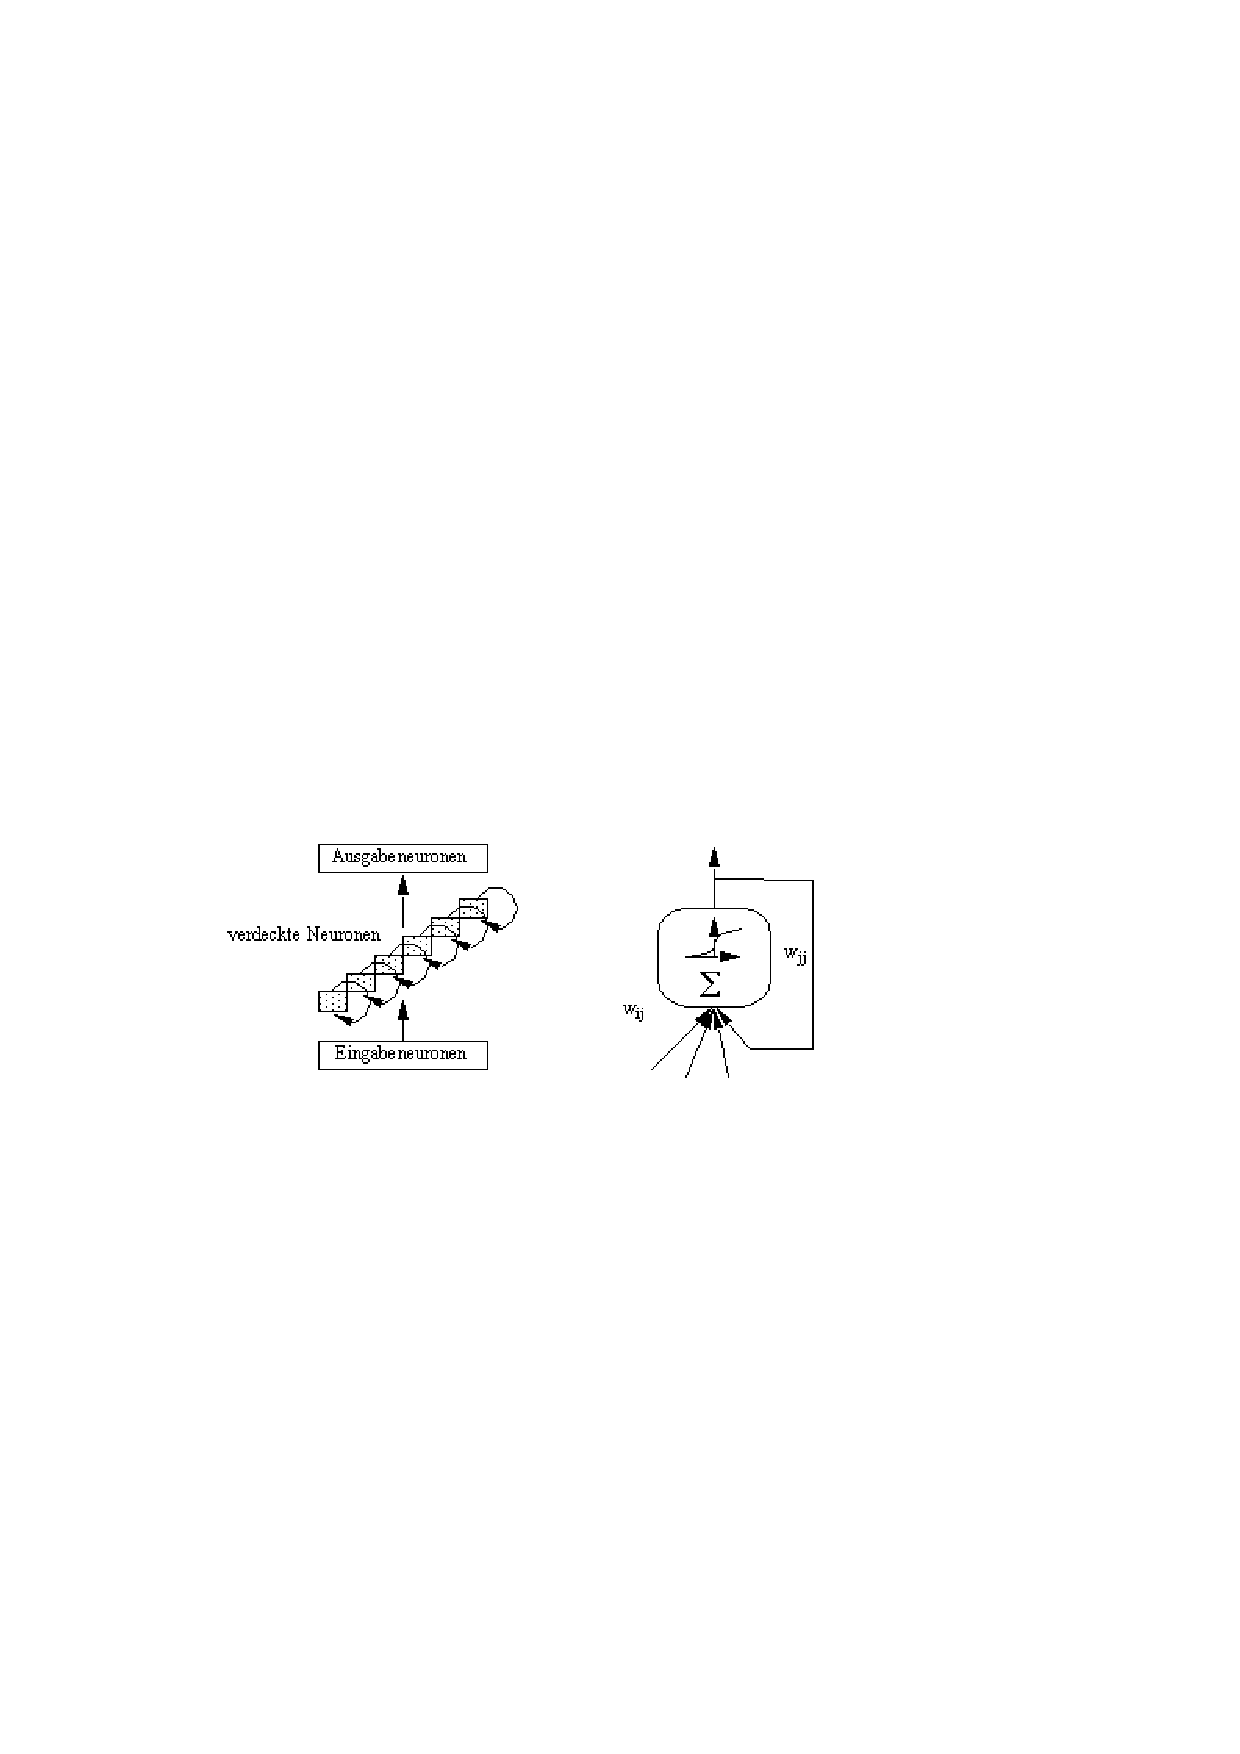
\includegraphics[width=\linewidth]{figures/ch06_rcc.pdf}
	\caption{Architektur rekurrenter Cascade-Correlation-Netze (links) und ein Kandidatenneuron $j$ mit einer rekurrenten Verbindung zu sich selbst (rechts).}
	\label{fig:ch06_2-rcc}
\end{figure}


\subsubsection*{Training}
Das Verhalten eines Kandidatenneurons mit rekurrenter Verbindung zu sich selbst ist im Folgenden aufgeführt.

\begin{itemize}
	\item \emph{stark positives} Gewicht $w_{jj}$ - Das Kandidatenneuron fungiert als Flip-Flop: Es versucht seinen Zustand beizubehalten, wenn er nicht durch eine starke Netzeingabe geändert wird.
	\item \emph{stark negatives} Gewicht $w_{jj}$ - Das Kandidatenneuron oszilliert bei jedem Zeitschritt zwischen positiver und negativer Ausgabe. 
\end{itemize}

Sobald das Kandidatenneuron dem aktiven Netzwerk hinzugefügt wird, wird sein rekurrentes Gewicht ebenso wie die anderen Eingangsverbindungen eingefroren. Auf diese Art und Weise kann jedes verdeckte Neuron als eine Zustandsvariable in einem endlichen Automaten angesehen werden, der speziell für diese Aufgabe gebaut wurde.

Fahlman verwendet meistens die Funktion $f_{act}(x) = tanh(x)$ als Aktivierungsfunktion.
Während der Trainingsphase werden alle Gewichte $w_{ij}$ so geändert, dass sie die Korrelation des Kandidatenneurons mit dem Restfehler maximieren. Dies erfordert die Berechnung der Ableitung der Ausgabe nach den Gewichten $w_{ij}$ und $w_{jj}$:
\begin{align*}
	\frac{\partial}{\partial w_{ij}} o_j(t) &= 
		f'_{act}(net_j) \Big( o_i(t) + 
			\frac{\partial}{\partial w_{ij}} o_j(t-1) w_{jj} \Big)
			\quad i \ne j \\
	\frac{\partial}{\partial w_{jj}} o_j(t) &= 
		f'_{act}(net_j) \Big( o_j(t-1) + 
			\frac{\partial}{\partial w_{jj}} o_j(t-1) w_{jj} \Big)	
\end{align*}
\noindent
Der Term ganz rechts in den Gleichungen gibt den Einfluss des betreffenden Gewichts auf den vorigen Zustand des Neurons an. Da der Wert von im vorhergehenden Schritt berechnet wurde, kann er einfach gespeichert werden und im aktuellen Schritt verwendet werden.

Damit benötigt die rekurrente Version des Verfahrens die Speicherung eines weiteren Wertes für jedes Gewicht und der alten Aktivierung $o_j(t-1)$ des Neurons. Zum Zeitpunkt $t=0$ werden die Ausgaben der Neuronen und alle partiellen Ableitungen als Null angenommen.

In den Benchmarks zeigte sich, dass RCC für die untersuchten Aufgaben leistungsfähiger als Standard-Elman-Netze war, während sich RTRL als etwa gleich leistungsfähig im Vergleich, aber komplexer und für größere Netze als weniger gut geeignet herausstellte.

